\chapter{Resultados}
	
	Los datos utilizados fueron obtenidos de \textit{NASA Langley Research Center (LaRC) POWER Project} financiado por el Programa de Ciencias de la Tierra/Ciencias Aplicadas de la NASA.
	
	\begin{figure}[H]
		\centering
		\begin{subfigure}[t]{0.45\linewidth}
			\centering
			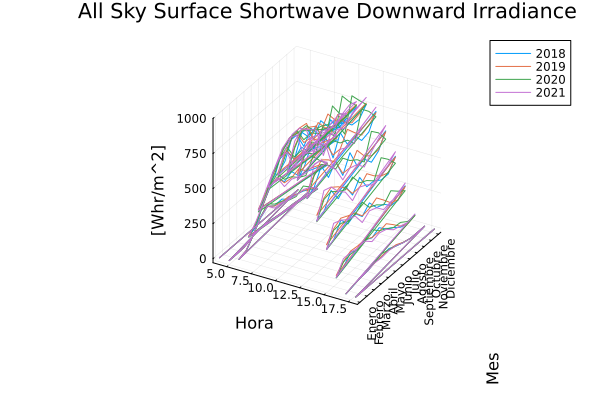
\includegraphics[
				width=\linewidth,
				height = 60mm,
				keepaspectratio
			]{Resultados/DataAnalysis/ALLSKY_SFC_SW_DWN_3d.png}
			\caption{Irradiación de onda corta promedio bajo todas las condiciones climáticas sobre el lugar seleccionado}
			\label{fig:ALLSKY_SFC_SW_DWN_3d}
		\end{subfigure}
		\hfill
		\begin{subfigure}[t]{0.45\linewidth}
			\centering
			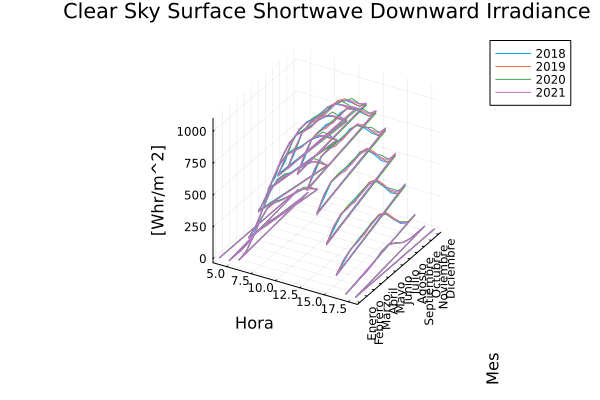
\includegraphics[
				width=\linewidth,
				height = 60mm,
				keepaspectratio
			]{Resultados/DataAnalysis/CLRSKY_SFC_SW_DWN_3d.png}
			\caption{Irradiación de onda corta promedio únicamente en cielo despejado sobre el lugar seleccionado}
			\label{fig:CLRSKY_SFC_SW_DWN_3d}
		\end{subfigure}
	\end{figure}
	\begin{figure}[H]\ContinuedFloat
		\begin{subfigure}[t]{0.45\linewidth}
			\centering
			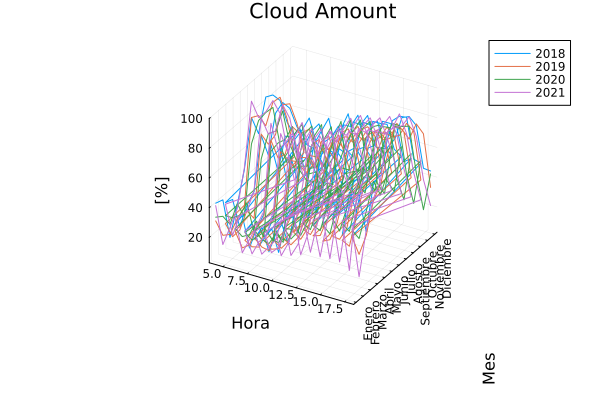
\includegraphics[
				width=\linewidth,
				height = 60mm,
				keepaspectratio
			]{Resultados/DataAnalysis/CLOUD_AMT_3d.png}
			\caption{Cantidad de nubes promedio sobre el lugar selccionado}
			\label{fig:CLOUD_AMT_3d}
		\end{subfigure}
		\hfill
		\begin{subfigure}[t]{0.45\linewidth}
			\centering
			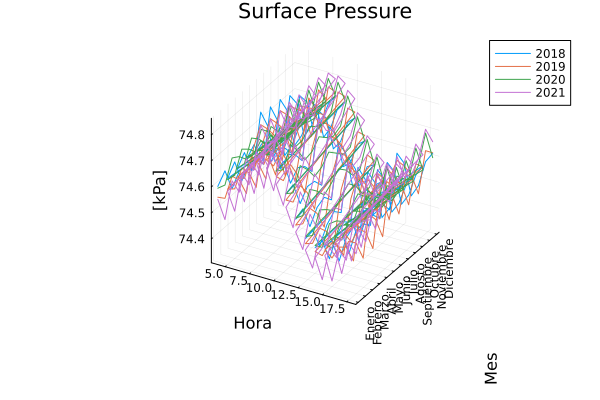
\includegraphics[
				width=\linewidth,
				height = 60mm,
				keepaspectratio
			]{Resultados/DataAnalysis/PS_3d.png}
			\caption{Presión superficial promedio sobre el lugar seleccionado}
			\label{fig:PS_3d}
		\end{subfigure}
	\end{figure}
	\begin{figure}[H]\ContinuedFloat
		\begin{subfigure}[t]{0.45\linewidth}
			\centering
			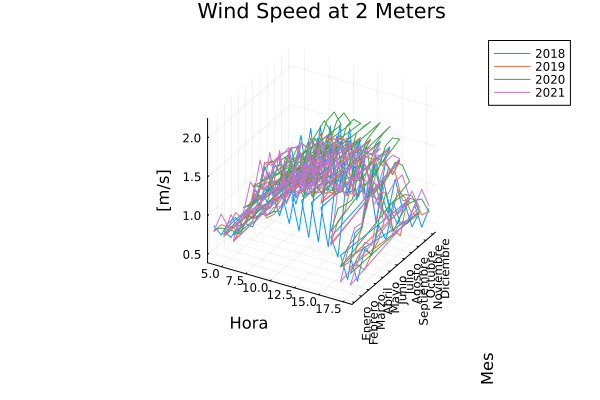
\includegraphics[
				width=\linewidth,
				height = 60mm,
				keepaspectratio
			]{Resultados/DataAnalysis/WS2M_3d.png}
			\caption{Rapidez promedio del viento sobre el lugar seleccionado}
			\label{fig:WS2M_3d}
		\end{subfigure}
		\begin{subfigure}[t]{0.45\linewidth}
			\centering
			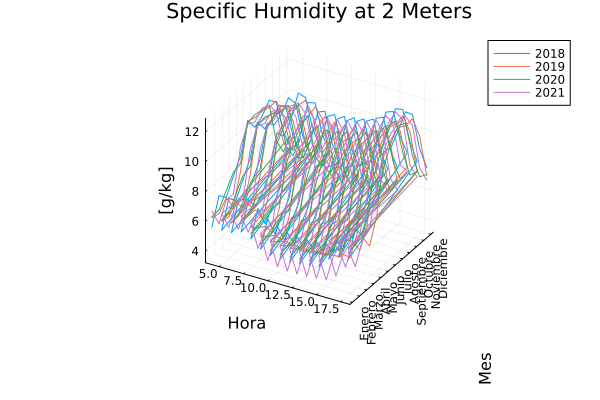
\includegraphics[
				width=\linewidth,
				height = 60mm,
				keepaspectratio
			]{Resultados/DataAnalysis/QV2M_3d.png}
			\caption{Humedad específica promedio a 2 metros sobre la superficie del lugar seleccionado}
			\label{fig:QV2M_3d}
		\end{subfigure}
	\end{figure}
	\begin{figure}[H]\ContinuedFloat
		\begin{subfigure}[t]{0.45\linewidth}
			\centering
			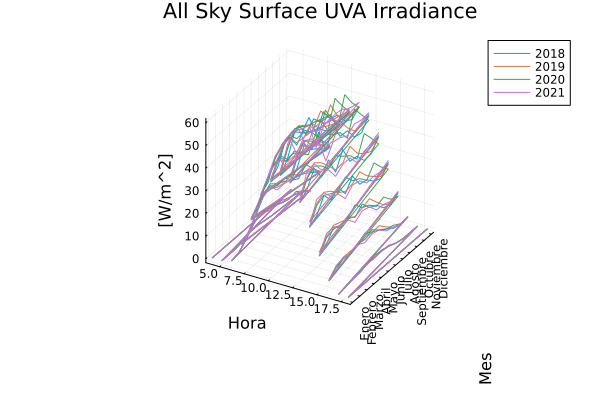
\includegraphics[
				width=\linewidth,
				height = 60mm,
				keepaspectratio
			]{Resultados/DataAnalysis/ALLSKY_SFC_UVA_3d.png}
			\caption{Irradiación UV tipo A bajo todas las condiciones climáticas sobre el lugar seleccionado}
			\label{fig:ALLSKY_SFC_UVA_3d}
		\end{subfigure}
		\hfill
		\begin{subfigure}[t]{0.45\linewidth}
			\centering
			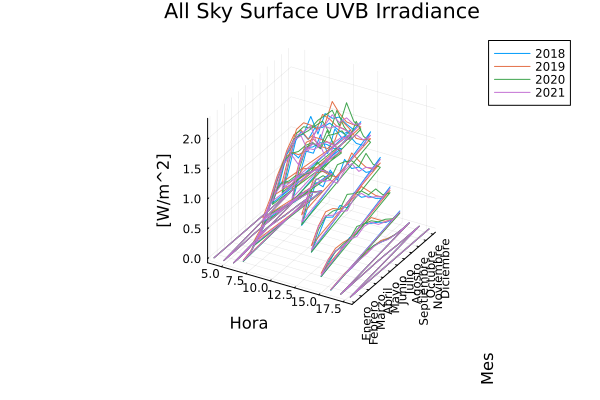
\includegraphics[
				width=\linewidth,
				height = 60mm,
				keepaspectratio
			]{Resultados/DataAnalysis/ALLSKY_SFC_UVB_3d.png}
			\caption{Irradiación UV tipo B bajo todas las condiciones climáticas sobre el lugar seleccionado}
			\label{fig:ALLSKY_SFC_UVB_3d}
		\end{subfigure}
		\caption{Gráficas obtenidas de la propuesta de la~\cref{sec:ch6-lugar-fisico}}
	\end{figure}